\documentclass[12pt]{article}
\usepackage{mathtools}
\usepackage{amsfonts}
\usepackage[ngerman]{babel}
\usepackage[utf8]{inputenc}
\usepackage{hyperref}
\usepackage{graphicx}
\usepackage{float}
\usepackage{wrapfig}
\usepackage{textgreek}

\addto\captionsngerman{
  \renewcommand{\figurename}{Abb.}
} 

\title{Quaternionen mit Java}
\author{Christian Basler}
\date{}

\begin{document}
  \maketitle

\begin{figure}[h]
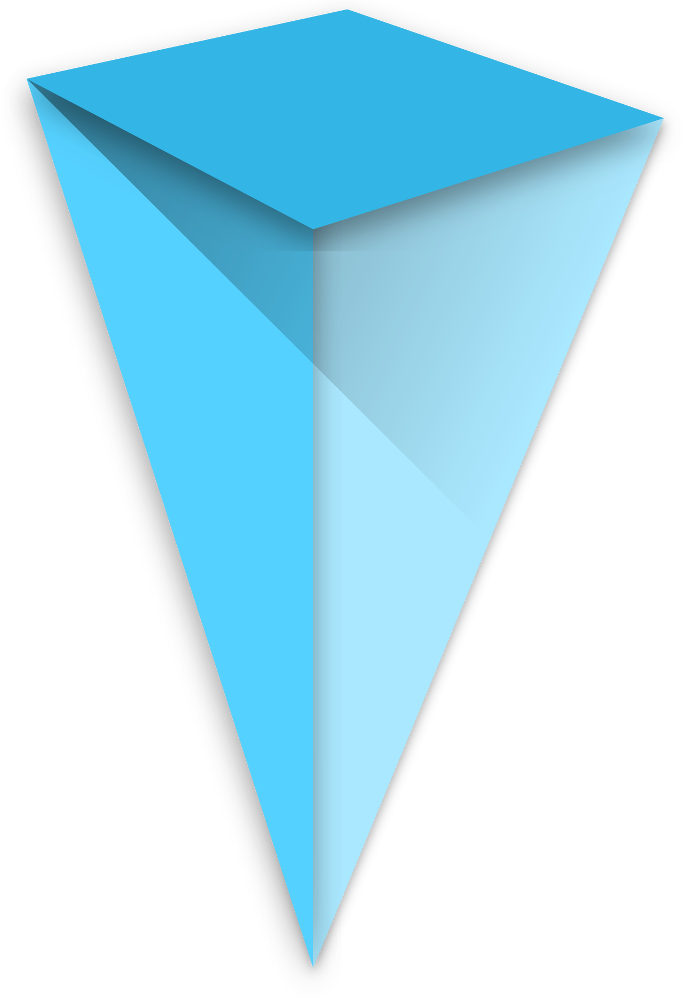
\includegraphics[width=0.2\textwidth]{logo.png}
\centering
\end{figure}

  \tableofcontents

  \section{Zusammenfassung}



  \section{Grundlagen}

  Quaternionen $\mathbb{H}$ erweitern die Komplexen Zahlen $\mathbb{C}$ um die Komponenten $\mathrm{j}$ und $\mathrm{k}$, so dass
  $$ q = q_0 + q_1 \mathrm{i} + q_2 \mathrm{j} + q_3 \mathrm{k} $$
  Dabei gilt $\mathrm{i}^2 = \mathrm{j}^2 = \mathrm{k}^2 = \mathrm{i}\mathrm{j}\mathrm{k} = -1$ und daher auch z.B. $\mathrm{i}\mathrm{j} = \mathrm{k}$ und $\mathrm{j}\mathrm{k} = \mathrm{i}$.

  Euklidische Vektoren können dabei wie folgt in eine Quaternion abgebildet werden:
  $$ q_{\vec{v}} = 0 + v_x \mathrm{i} + v_y \mathrm{j} + v_z \mathrm{k} $$
  Daher wird der Imaginärteil einer Quaternion auch Vektorteil genannt. Eine solche Quaternion, welche nur aus Vektorteil besteht, wird auch als \textit{reine Quaternion} bezeichnet.


  \subsection{Polardarstellung und Rotation}

  Ist eine Quaternion $q \notin \mathbb{R}$, so lässt sie sich eindeutig in der Form
  $$ q = \lvert q \rvert (\cos{\phi} + \epsilon \sin{\phi}) $$
  darstellen mit dem Betrag
  $$ \lvert q \rvert = \sqrt{q_0^2 + q_1^2 + q_2^2 + q_3^2} $$
  dem Polarwinkel
  $$ \phi := \arccos{q} = \arccos{\mathrm{Re} q} $$
  und der reinen Einheitsquaternion
  $$ \epsilon = \frac{\mathrm{Im} q}{\lvert \mathrm{Im} q \rvert} $$

  Dies ermöglicht eine  elegante Darstellung von Drehungen im dreidimensionalen Raum mittels Einheitsquaternionen:
  \begin{align*}
    y &= q x q^{-1} = q x \bar{q} \\
	q &= \cos{\frac{\alpha}{2}} + \epsilon \sin{\frac{\alpha}{2}}
  \end{align*}
  $q$ ist dabei eine Einheitsquaternion\footnote{$\lvert q \rvert = 1$} und stellt zusammen mit $\bar{q}$ eine Drehung um Achse $\epsilon$ mit Winkel $\alpha$ dar.


  \section{Java-Bibliothek}

  Die Java-Bibliothek stellt eine Klasse \texttt{Quaternion} mit den darauf möglichen Operatoren zur Verfügung\footnote{Die Operatoren und Methoden werden in Anhang A aufgelistet}. Die Quaternionen sind unveränderlich, jede Operation erzeugt folglich eine neue Quaternion.

  Aufgrund der Einschränkungen von Java sind alle Operationen als Methoden implementiert, $\bar{q}$ heisst also beispielsweise \texttt{q.conjugate()}.

  Etwas speziell sind die folgenden Methoden:
  \begin{itemize}
    \item \texttt{q.norm()}: gibt im Gegensatz zu den anderen Methoden ein \texttt{double} zurück anstelle einer \texttt{Quaternion}. Ausserdem gibt es verschiedene Auffassungen, ob diese dem Betrag oder dem Quadrat des Betrags entsprechen soll. In meiner Implementierung entspricht sie dem Betrag.
    \item \texttt{q.rotate(\texttheta, x, y, z)}: ist eine Hilfsmethode, falls man nicht extra ein Quaternion erzeugen möchte um die Rotation zu definieren.
    \item \texttt{q.equals(r)}, \texttt{q.hashCode()}: da man \texttt{double}-Werte nicht direkt miteinander vergleichen kann, wird verglichen ob $\lvert \lvert q \rvert - \lvert r \rvert \rvert < \Delta$. Um dies genauer zu steuern kann das \textdelta auch als Argument mitgegeben werden. Da diese Art der Implementierung Probleme mit der Hash-Definition ergeben (\texttt{q.equals(r)} $\implies$ \texttt{q.hashCode() == r.hashCode()}).
    \item \texttt{q.getScaledRotation(s)}: ergibt ein Quaternion mit gleicher Drehachse und einem um $s$ gestreckten Winkel.
  \end{itemize}

  Zum Erstellen neuer Quaternionen besteht ausserdem die statische Methode \texttt{H}, was die elegante Schreibweise \texttt{q = H(1, 3, 2, 5); v = H(1, 1, 0); x = H(42)} erlaubt. 

  Für Fälle wo euklidische Vektoren benötigt werden, z.B. beim Konstruktor für die Rotation \texttt{H($\alpha$, $\vec{v}$)}, gibt es ausserdem die Klasse \texttt{Vector}, welche jedoch nur sehr eingeschränkte Funktionalität bietet. Vektoren können mit der statischen Methode \texttt{V} analog zu den Quaternionen erstellt werden.

\newpage
  \section{Beispielanwendungen}
  \subsection{Wo ist unten?}

\begin{wrapfigure}{R}{0.4\textwidth}
    \vspace{-12pt}
    \centering
    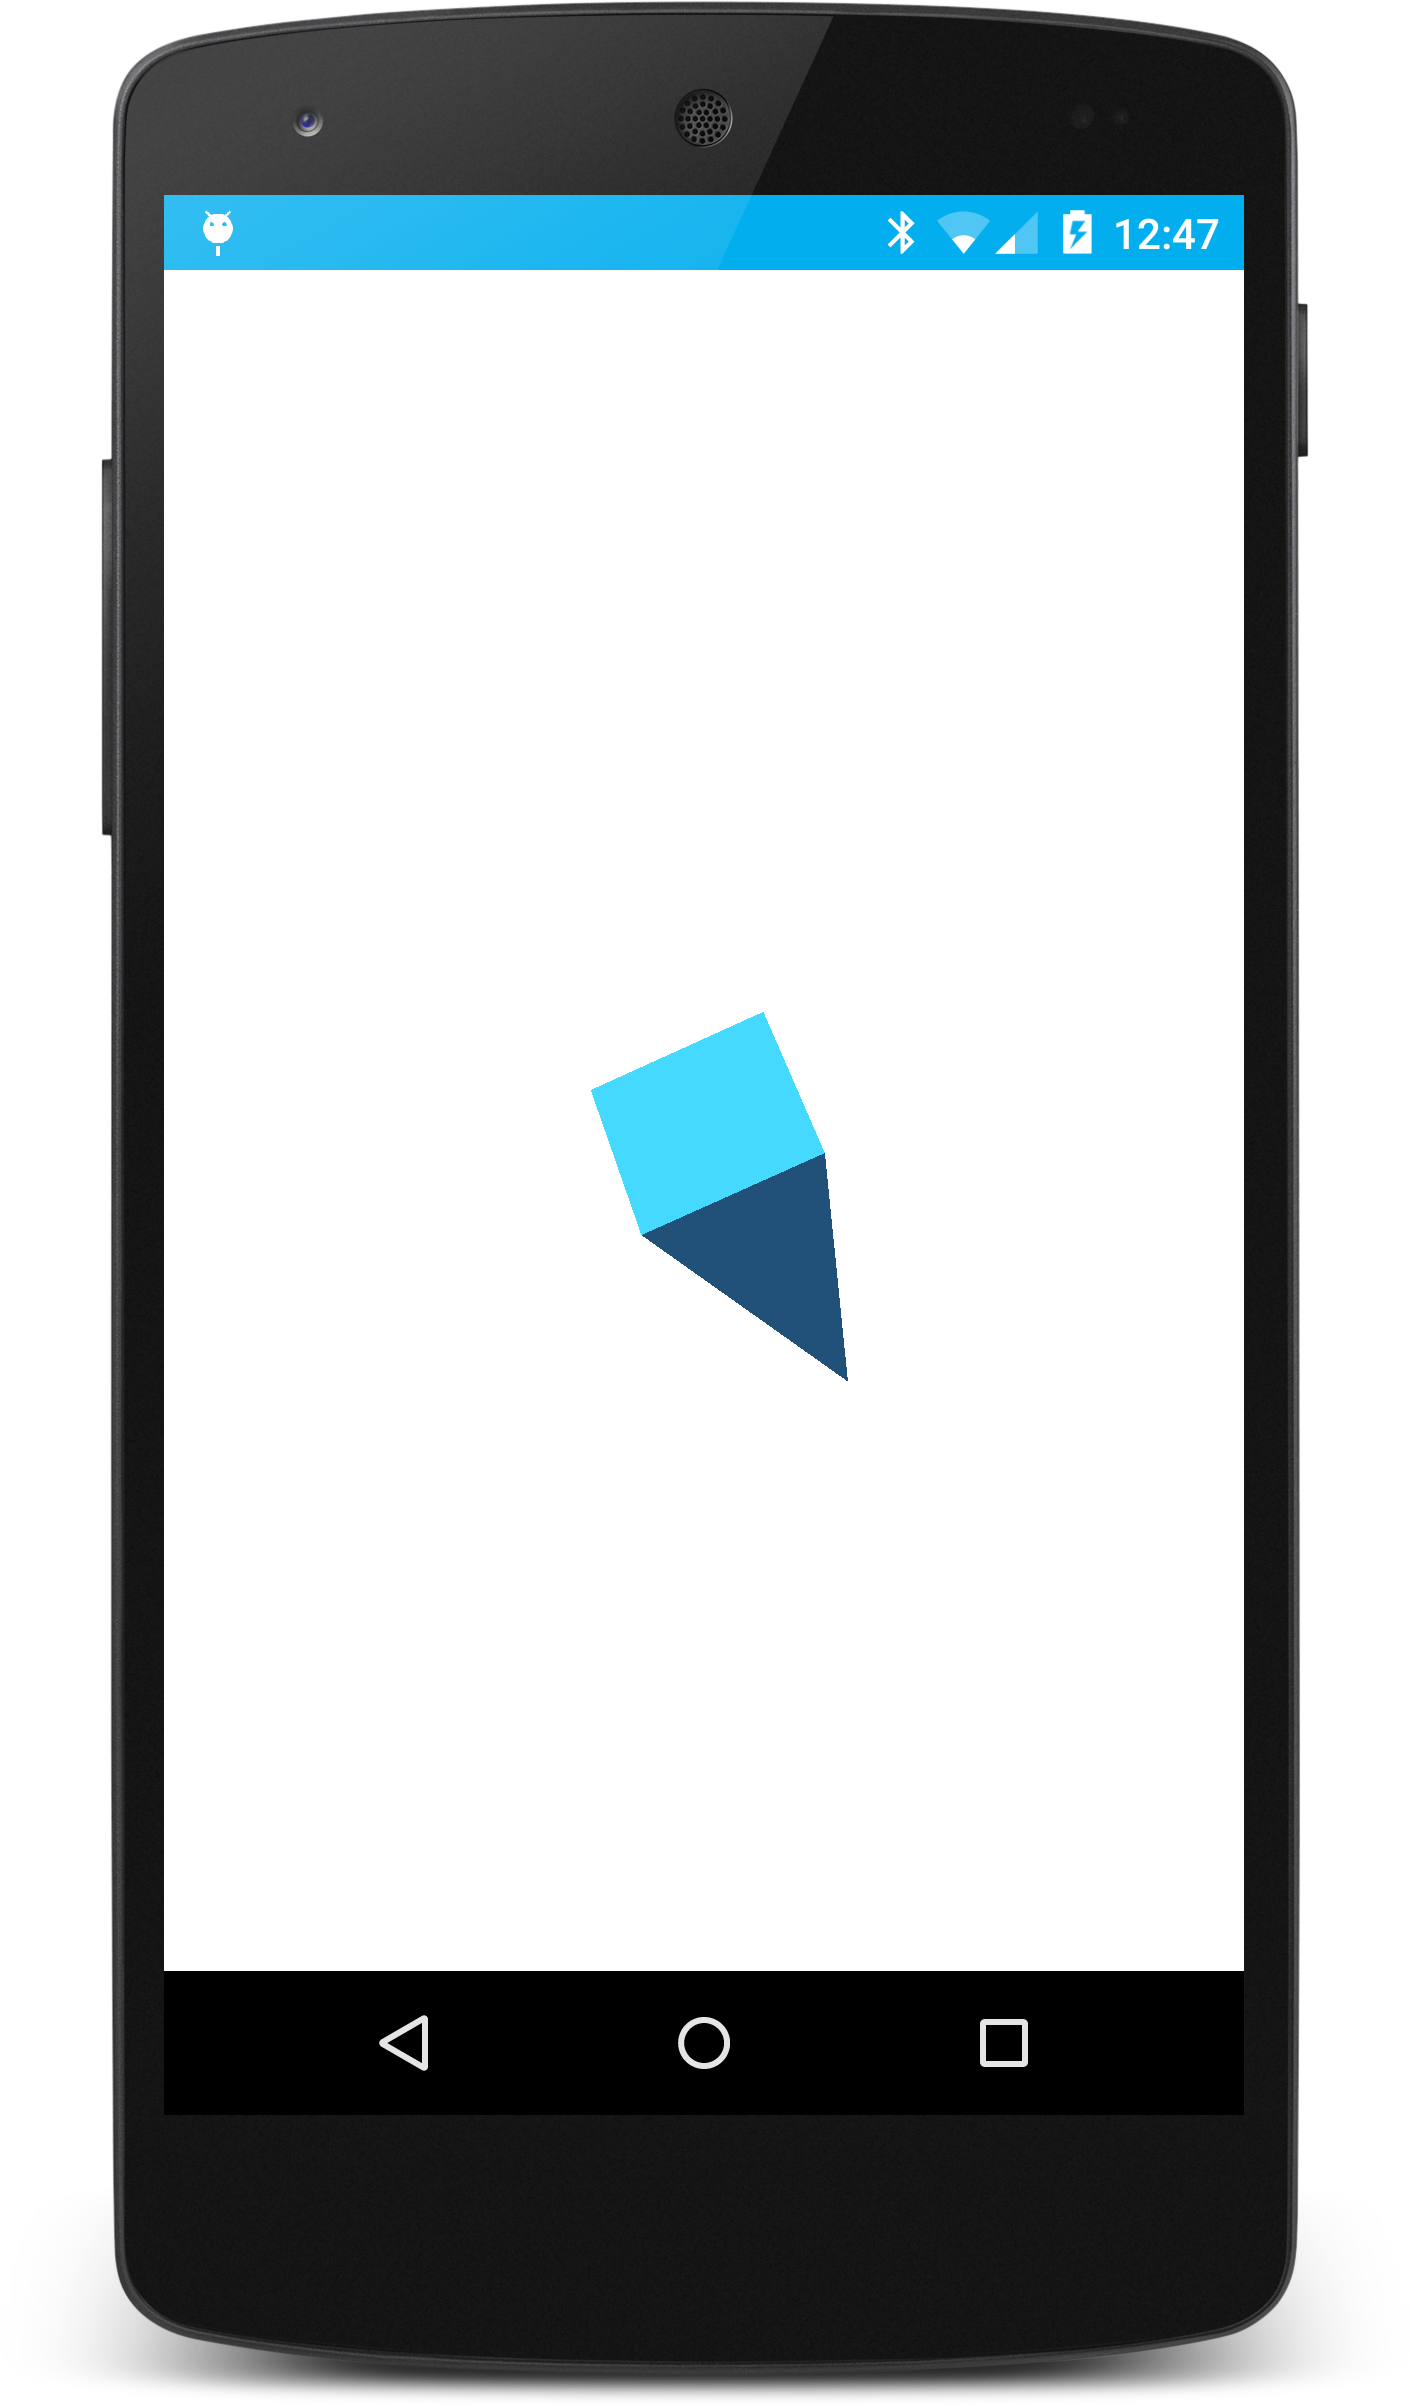
\includegraphics[width=0.4\textwidth]{down.png}
    \vspace{-18pt}
    \caption{Wo ist unten?}
    \label{fig:screenshot_down}
\end{wrapfigure}
  Die App soll immer nach unten zeigen. Dazu gibt es bei modernen Smartphones grundsätzlich zwei Sensoren, den Beschleunigungssensor und das Gyroskop. Ersterer misst unter anderem die Erdbeschleunigung, zeigt also recht schön nach unten. Allerdings verhällt er sich sehr nervös bei den geringsten Erschütterungen. Das Gyroskop misst
Winkelgeschwindigkeiten entlang der drei Achsen, aus welchen man die Lage, und damit auch ``unten'' rekonstruieren kann. Da dabei viele aufeinanderfolgende Messwerte multipliziert werden, entsteht ein sogenannter Drift, das heisst ``unten'' zeigt plötzlich irgendwo anders hin.

  Um ein gutes Resultat zu erhalten, muss man deshalb die Messungen der beiden Instrumente kombinieren. Der Beschleunigungssensor soll helfen, den Drift zu vermeiden, und das Gyroskop soll den Beschleunigungssensor stabilisieren. Dazu werden die Daten des Beschleunigungssensors $a_t$ mit einem Tiefpass gefiltert und für eine bessere Reaktion mit den Gyroskopdaten $r_t$ kombiniert. Werden dabei Quaternionen eingesetzt, können diese durchgehend verwendet werden\footnote{Ausser beim Auslesen und bei der Arbeit mit der 3D-Bibliothek Rajawali, wo Eulersche Winkel verlangt werden.}. Im Wesentlichen sieht dies so aus:
  \begin{align*}
    a' &= a C_{LPF} +  a_t (1 - C_{LPF}) \\
    g' &= r_t g \bar{r_t}    \\
    f' &= (1 - C_{SFF}) a' + C_{SFF} g'
  \end{align*}
  Wobei der Koeffizient für den Tiefpassfilter $C_{LPF}$ und derjenige für den Sensorfusion-Filter $C_{SFF} \in \mathbb{R}$.


  \subsection{Künstlicher Horizont}

\begin{wrapfigure}{L}{0.4\textwidth}
    \vspace{-12pt}
    \centering
    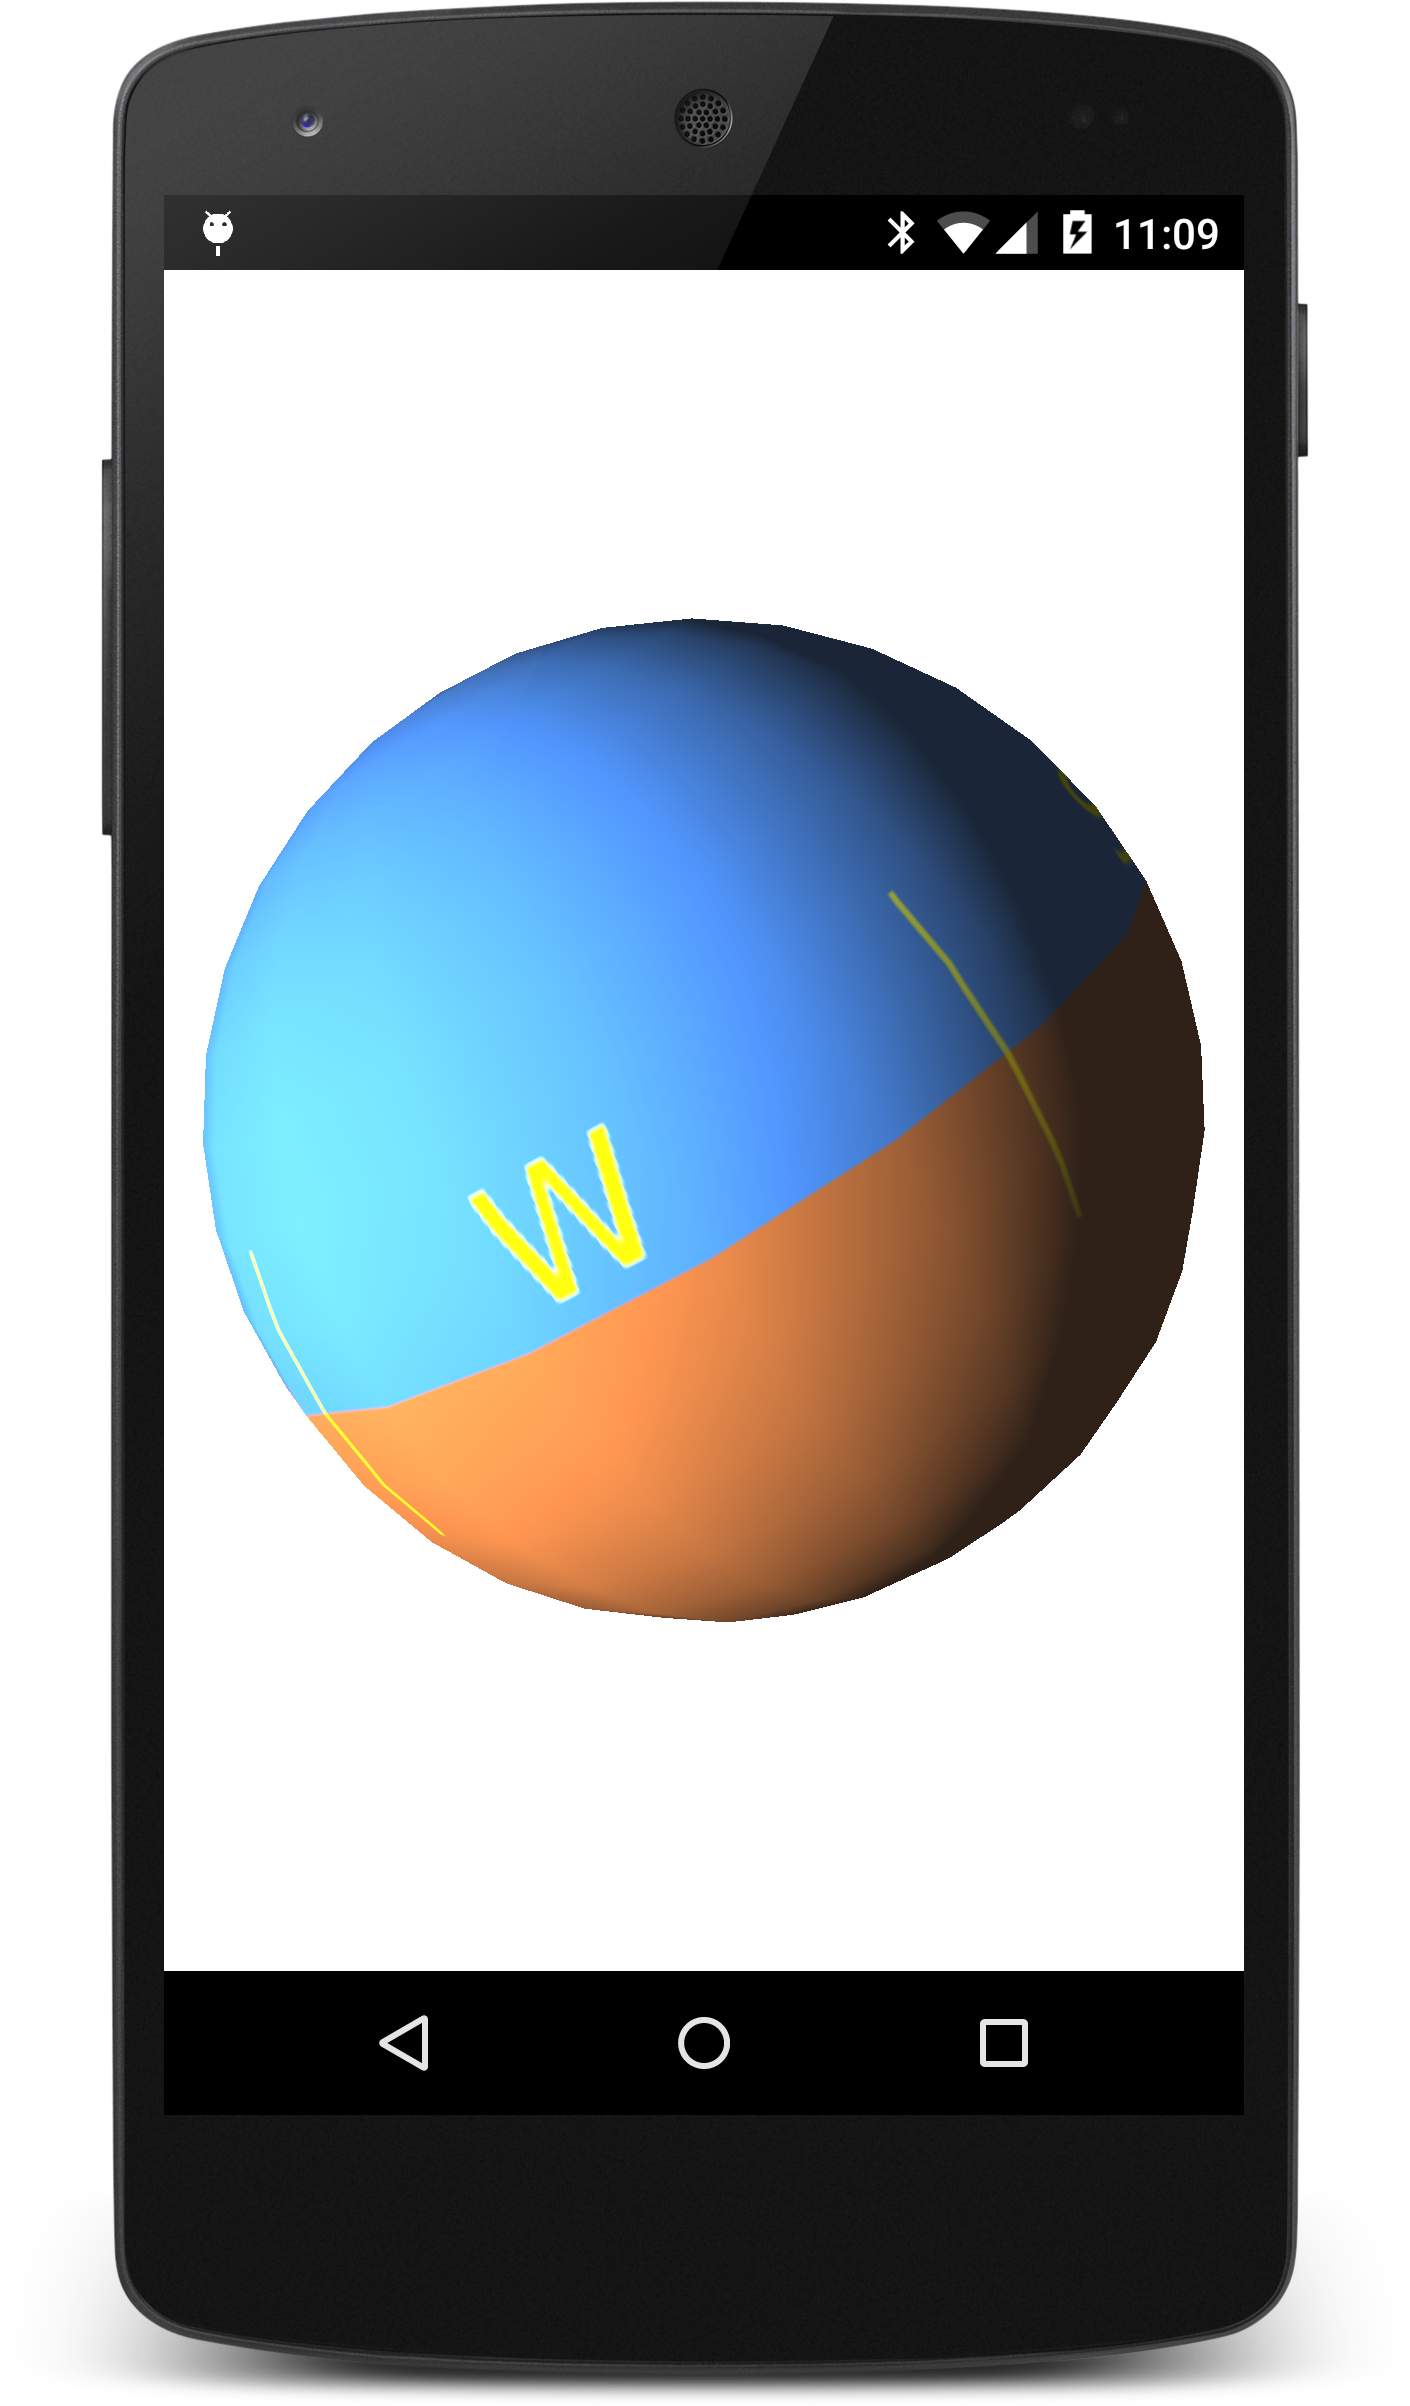
\includegraphics[width=0.4\textwidth]{artificial-horizon.png}
    \vspace{-18pt}
    \caption{Künstlicher Horizont}
    \label{fig:screenshot_artificial_horizon}
    \vspace{-10pt}
\end{wrapfigure}
  Eine Erweiterung der ersten App. Diese soll auch die Himmelsrichtung anzeigen, also die grundsätzliche Orientierung im Raum.

  Im gegensatz zur ersten App wurden hier nicht Vektoren fusioniert, sondern die Drehung von der Basisausrichtung (das Gerät liegt flach auf dem Tisch, mit der oberseite in Richtung Norden) zur tatsächlichen Ausrichtung. Dank der Methode \texttt{q.getScaledRotation(factor)}, im folgenden als $q_{factor}$ dargestellt, liess sich zumindest dies sehr elegant lösen:
  $$ f' = (f g)_{1-C_SFF} r_{C_{SFF}} $$
  Wobei $r$ die kombinierte Drehung von Kompass und Beschleunigungssensor ist.  Da hier schlussendlich doch eine Drehmatrix verwendet werden musste, machen die Quaternionen etwas weniger Sinn als beim ersten Beispiel\footnote{...oder ich habe einfach die elegante Lösung übersehen}.


  \section{Diskussion}

  Die Umsetzung der Quaternionen als Objekt war ziemlich einfach. Etwas schade ist nur, dass Java keine Möglichkeit bietet, beispielsweise Additionen als $a + b$ darzustellen anstatt \texttt{a.add(b)}. Ich habe mir deshalb auch überlegt die Bibliothek in Scala umzusetzen. Damit ist es aber nicht so einfach Apps zu schreiben, was den grössten Vorteil dieser Bibliothek wieder zunichte machen würde.

  Da bei den Android-Sensoren durchgehend Zahlen vom Typ \texttt{float} verwendet werden, habe ich mir auch überlegt eine Version zu machen die darauf basiert anstatt \texttt{double}, doch auf modernen Geräten scheinen die letzteren dank Hardwarebeschleunigung schneller zu sein, der Zusatzaufwand lohnt sich also vermutlich nicht.

  Die ``Wo ist unten''-App erwies sich als gutes Beispiel, wie einfach die Arbeit mit Quaternionen sein kann. Das grösste Problem war die Darstellung, mein Versuch mit OpenGL ist kläglich daran gescheitert dass ich ihm nicht beibringen konnte die richtigen Seiten zu zeichenen.

  Zuerst dachte ich, der künstliche Horizont wäre fast ein bisschen zu einfach nach ``Unten'', es ist ja schliesslich das gleiche Problem nur mit einer Drehung mehr. Ganz so einfach war es dann doch nicht, und ich musste auf eine Drehmatrix ausweichen. Ich vermute immer noch es geht auch einfacher, aber ich konnte die Lösung dazu nicht finden.


  \section{Literatur}

  Wikipedia ist immer wieder eine gute Anlaufstelle für mathematische Fragen. Insbesondere die englischsprachige Version behandelt Quaternionen sehr ausführlich.

  \begin{itemize}
    \item \url{http://de.wikipedia.org/wiki/Quaternion}
    \item \url{http://en.wikipedia.org/wiki/Quaternion}
    \item \url{http://en.wikipedia.org/wiki/Quaternions_and_spatial_rotation}
  \end{itemize}

  \appendix
  \addcontentsline{toc}{section}{Anhang}
  \section*{Anhang}
  \renewcommand{\thesubsection}{\Alph{subsection}}

  \subsection{Methoden der Klasse Quaternion}
  \begin{itemize}
    \item \texttt{q.add(r)} $= q + r$
    \item \texttt{q.subtract(r)} $= q - r$
    \item \texttt{q.multiply(r)} $= q r$
    \item \texttt{q.conjugate()} $= \bar{q}$
    \item \texttt{q.norm()} $= \lvert q \rvert$
    \item \texttt{q.normalize()} $= \frac{q}{\lvert q \rvert}$
    \item \texttt{q.reciprocal()} $= q^{-1}$
    \item \texttt{q.divide(r)} $= q r^{-1}$
    \item \texttt{q.rotate(r)} $= r q \bar{r}$
    \item \texttt{q.rotate($\theta$, x, y, z)} $=$ Rotation\ um\ Achse\ $(x, y, z)$ mit Winkel $\theta$
    \item \texttt{q.exp()} $= e^q$
    \item \texttt{q.ln()} $= \ln q$
    \item \texttt{q.dot(r)} $= q \cdot r = q_0 r_0 + q_1 r_1 + q_2 r_2 + q_3 r_3$
    \item \texttt{q.cross(r)} $= \vec{q} \times \vec{r}$ (d.h. $q_0$ und $r_0$ werden ignoriert)
    \item \texttt{q.getRe()} $= \mathbf{Re}\ q$
    \item \texttt{q.getIm()} $= \mathbf{Im}\ q$
    \item \texttt{q.getRotationAngle()} $= 2 cos^{-1}\frac{\mathbf{Re} q}{\lvert q \rvert}$
    \item \texttt{q.getRotationAxis()} $= \frac{\mathbf{Im}\ q}{\lvert \mathbf{Im} q \rvert}$
    \item \texttt{q.getScaledRotation(s)}
    \item \texttt{q.equals(r, $\delta$)} $= |q - r|^2 < \delta$
    \item \texttt{q.equals(r)} = q.equals(r, Quaternion.DELTA)
  \end{itemize}

  Zum Erstellen neuer Quaternionen besteht ausserdem die statische Methode \texttt{H} in folgenden Ausführungen:
  \begin{itemize}
    \item \texttt{H($q_0$, $q_1$, $q_2$, $q_3$)} $= q_0 + q_1 \mathrm{i} + q_2 \mathrm{j} + q_3 \mathrm{k}$
    \item \texttt{H(x, y, z)} $= x \mathrm{i} + y \mathrm{j} + z \mathrm{k}$
    \item \texttt{H(w)} $= w$
    \item \texttt{H($\alpha$, $\vec{v}$)} $= \cos\frac{\alpha}{2} + \mathrm{i} \sin\frac{\alpha}{2} v_x + \mathrm{j} \sin\frac{\alpha}{2} v_y + \mathrm{k} \sin\frac{\alpha}{2} v_z$
    \item H([x, y, z]), H([w, x, y, z])
    \item getRotation(p, q) $= r$, so dass $r p \bar{r} = q$
  \end{itemize}

  \subsection{}
  \begin{itemize}
    \item Java-Dokumentation siehe Ordner \texttt{javadoc}
    \item Sourcecode siehe Ordner \texttt{sources} oder
    \begin{itemize}
      \item \url{https://github.com/Dissem/MathLib}
      \item \url{https://github.com/Dissem/Down}
      \item \url{https://github.com/Dissem/Artificial-Horizon}
    \end{itemize}
  \end{itemize}

\end{document}